%\section{Paradigmi}

Gli elementi grafici e funzionali sono solo una parte dell'architettura del software di Metarace.
%
Un'altra componente importante dell'architettura di Metarace è che sfrutta il paradigma della programmazione guidata dagli eventi.
%
Nella programmazione guidata dagli eventi il flusso del programma è determinato da eventi esterni ad esso, come l'input di un utente o come un messaggio arrivato da un server.
%
Infatti Metarace ha una struttura capace di rispondere agli eventi avviati dal server ma anche agli eventi innescati dall'utente.
%
Il software presenta un'interfaccia utente che permette al giocatore di avviare una partita e, dato che esistono diverse tipologie di partite, di scegliere la tipologia di gara a cui partecipare.
%
L'insieme degli eventi che possono verificarsi è stato scelto in fase di elaborazione ed è costituito da 13 eventi.
%
Parte del mio lavoro è stato la progettazione e l'implementazione di 9 di questi, che sono: PlayEvent, AvailableRacesEvent, JoinEvent, PlayerJoinedEvent, StartingGridEvent, AnotherPlayerJoinedEvent, CountdownEvent, RaceEvent, LeaderboardEvent.

%\section{Model - View - Controller (MVC)}
\section{L'architettura di Metarace}

Un videogioco è un applicativo che è particolarmente adatto alla divisione a strati.
%
Infatti l'architettura di Metarace può essere divisa in vari strati che si occupano del suo funzionamento.
%
È possibile individuare lo strato della Logica Implementativa, lo strato del Network, lo strato dell'Interfaccia Grafica e lo strato dell'Interfaccia Utente (UI).

\begin{description}
    \item[Lo strato della Logica Implementativa] è composto da tutti gli script che permettono il funzionamento dell'applicazione.
    \item[Lo strato del Network] permette di comunicare da e verso il server e di tradurre queste comunicazioni in istruzioni per lo strato della Logica Implementativa.
    \item[Lo strato dell'Interfaccia Grafica] è composto dall'engine di gioco e da tutti gli elementi che vengono renderizzati a schermo.
    \item[Lo strato della UI] permette di catturare l'input dato dall'utente e di tradurlo in rispettivi eventi di gioco.
\end{description}

\begin{figure}[!ht]
    \centering
    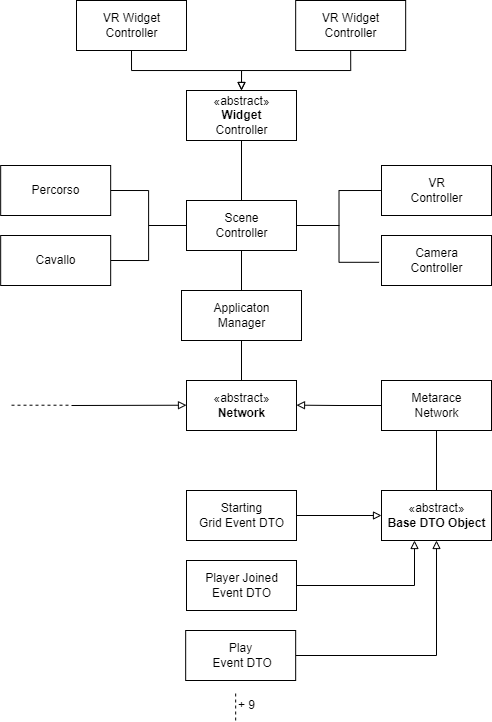
\includegraphics[width=12cm]{figure/Modello_di_Dominio_Metarace.drawio.png}
    \caption{Modello di Dominio parziale per Metarace}
    \label{img:Dominio}
\end{figure}

    \subsection{Progettazione guidata dalle responsabilità}

    Nella progettazione guidata dalle responsabilità gli oggetti software sono considerati come dotati di responsabilità, di ruoli e di collaborazioni.
    %
    Sulla base del modello di dominio  parziale mostrato in Figura \ref{img:Dominio} vengono assegnate le responsabilità di ciascun oggetto.

    Le responsabilità sono di due tipi: \textit{Responsabilità di fare} e \textit{Responsabilità di conoscere}.
    %
    Un importante tipo di responsabilità di fare è quella del pattern \textit{Creator}.
    %
    La maggiorparte delle responsabilità di questo tipo sono state assegnate all'oggetto \textit{Application Manager}.  
    %
    Questo è anche dovuto dal fatto che nel momento in cui il gioco viene fatto partire, un attore deve essere già in scena per poter instanziare tutti gli altri Actor.
    %
    Questo attore è proprio l'\textit{Application Manager}.

    Un'altro importante pattern da seguire quando si assegnano le responsabilità è il pattern \textit{Low Coupling}.
    %
    Questo pattern punta a cercare il progetto che abbia il minor livello di accoppiamento.
    %
    Per tenere l'accoppiamento basso in Metarace è stato sfruttato uno strumento offerto da Unreal Engine: i delegates.

    I delegates permettono di chiamare funzioni di oggetti C++ in modo generico e type-safe \cite{UDelegates}.
    %
    Un delegate può essere legato dinamicamente ad una funzione di un oggetto scelto e permette di eseguire questa funzione in un momento futuro senza che il chiamante debba conoscere il tipo dell'oggetto chiamato.
    %
    Questo strumento riduce di molto l'accoppiamento in quanto in questo modo due oggetti possono collaborare senza conoscersi.

    \subsection{L'\textit{Application Manager}}

    L'Application Manager è l'unica classe già presente in scena durante la prima chiamata alla funzione \textit{Begin Play}.
    %
    In Unreal Engine è possibile posizionare una classe C++ nel mondo di gioco attraverso la creazione di un Blueprint sulla base di essa.
    %
    Allo stesso modo all'interno di una classe C++ è possibile avere dei riferimenti ad altri Blueprint basati sempre su classi C++.
    %
    Infatti, Unreal Engine permette di creare questo tipo di riferimenti attraverso il template di classe \textit{TSubclassOf<T>}.

    \begin{lstlisting}[caption = Sezione dell'header file della classe ApplicationManager dove vengono referenziate altri Blueprint basati su classi C++]
#include ...

UCLASS()
class Metarace AMetaraceApplicationManager : public AActor
{
    [...] //Costruttore di classe, funzione BeginPlay e Tick

protected:
    UPROPERTY(Category=TableController, EditAnywhere, BlueprintReadWrite)
    TSubclassOf<AMetaraceSceneController> SceneControllerBP;
    UPROPERTY(Category=TableController, EditAnywhere, BlueprintReadWrite)
    TSubclassOf<AMetaraceNetworkActor> NetworkActorBP;

private:
    UPROPERTY()
    AMetaraceSceneController* SceneController = nullptr;
    UPROPERTY()
    AMetaraceNetworkActor* NetworkActor = nullptr;
};        
    \end{lstlisting}

    Nella funzione \textit{Begin Play} viene messo in pratica il pattern \textit{Create} per gli oggetti SceneController e NetworkActor:

    \begin{lstlisting}[caption = Sezione del file source dell'Application Manager dove vengono creati gli oggetti SceneController e NetworkActor]
void AMetaraceApplicationManager::BeginPlay()
{
    Super::BeginPlay();

    UWorld* World = GetWorld();
    if(!World) { return; }

    FActorSpawnParameters SpawnParams;
    if(SceneControllerBP)
    {
        SceneController = World->SpawnActor<AMetaraceSceneController>(
            SceneControllerBP, GetTransform(), SpawnParams);
    }
    if(NetworkActorBP)
    {
        NetworkActor = World->SpawnActor<AMetaraceNetworkActor>(
            NetworkActorBP, GetTransform(), SpawnParams);
        NetworkActor->Initialize();
    }

    \end{lstlisting}

    L'ApplicationManager si occupa anche di creare i Bind per tutti i delegate visto che già ha i riferimenti a tutti gli oggetti che li utilizzano.

    \label{alg:bindDelegate}
    \begin{lstlisting}[firstnumber=22, caption = Sezione del file source dell'Application Manager dove viene formato il Bind dei delegates]

    if(SceneController && NetworkActor)
    {
        SceneController->OnWantToSendMessage.
            BindUObject(NetworkActor, 
                &MetaraceNetworkActor::SendMessage);
        SceneController->WidgetController->OnWantToSendMessage.
            BindUObject(NetworkActor, 
                &AMetaraceNetworkActor::SendMessage);

        NetworkActor->OnAvailableRacesFormatsEventDelegate.
            BindUObject(SceneController,
                &AMetaraceSceneController::ShowAvailableRaceFormats);
        NetworkActor->OnPlayerJoinedEventDelegate.
            BindUObject(SceneController,
                &AMetaraceSceneController::PlayerJoined);
        NetworkActor->OnStartingGridEventDelegate.
            BindUObject(SceneController,
                &AMetaraceSceneController::StartingGrid);
        NetworkActor->OnRaceEventDelegate.
            BindUObject(SceneController,
                &AMetaraceSceneController::InitRace);
        NetworkActor->OnCountdownEventDelegate.
            BindUObject(SceneController,
                &AMetaraceSceneController::ShowCountDown);
        NetworkActor->OnAnotherPlayerJoinedEventDelegate.
            BindUObject(SceneController,
                &AMetaraceSceneController::AnotherPlayerJoined);
        NetworkActor->OnLeaderboardEventDelegate.
            BindUObject(SceneController,
                &AMetaraceSceneController::OnLeaderboardEvent);
    }
}        
    \end{lstlisting}

    Lo SceneController possiede un delegate perché a gara finita deve poter inviare il file \textit{Json} per l'evento \textit{RaceFinischedEvent} verso il server.
    %
    Il WidgetController anche possiede un delegate perché deve poter inviare messaggi verso il server dato che è lui che si occupa degli eventi \textit{PlayEvent} e \textit{JoinEvent}.
    %
    NetworkActor possiede inoltre un delegate per ogni evento che deve gestire e viene creato il Bind con lo SceneController per delegare quest'ultimo a eseguire la logica implementativa.

    Dopo l'esecuzione della funzione \textit{Begin Play} l'ApplicationManager non viene più chiamato.

    \subsection{Lo \textit{SceneController}}

    Lo \textit{SceneController} è la classe che si interfaccia con lo strato di Logica Implementativa e con lo strato dell'Interfaccia Utente.
    %
    A questa classe sono state assegnate le responsabilità di conosce gli oggetti più importanti nel livello di gioco: conosce il percorso di gara e fa comparire i cavalli dei giocatori inizializzando i loro dati.
    %
    Inoltre si occupa della creazione delle classi WidgetController, CameraController e VRController.

\section{Architettura Client - Server e la WebSocket}

Metarace è quindi un applicativo con struttura client-server e si collega al server con un canale di comunicazione bidirezionale basato sul protocollo WebSocket.
%
Questo protocollo è stato scelto per due motivi: il primo è che permette di tenere aperta una connessione tra client e server fino a che non viene terminata da uno dei due partecipanti; il secondo è che non è necessario definire il protocollo di comunicazione dato che si basa sul diffuso protocollo TCP.

Questo protocollo trasferisce i dati su una connessione full-duplex su singolo socket e permette l'invio e la ricezione di messaggi da parte di ambedue gli endpoint. 
%
Una connessione WebSocket è instaurata con un handshake specifico basato sul protocollo HTTP.
%
A seguito di questo handshake il protocollo di comunicazione cambia, e passa da HTTP a WebSocket tramite la connessione TCP utilizzata inizialmente. 

Unreal Engine fornisce supporto per l'utilizzo dei WebSocket tramite il modulo \textit{IWebSocket} \cite{UWebSocket}. Per poter utilizzare questo modulo bisogna aggiungere la dependency all'interno del file ".build.cs". Qui è mostrato il codice con l'aggiunta di tutte le dependencies utilizzate nel progetto:

\begin{lstlisting}[caption = Metarace.build.cs file]
using UnrealBuildTool;

public class Metarace : ModuleRules
{
	public Metarace(ReadOnlyTargetRules Target) : base(Target)
	{
		PublicDependencyModuleNames.AddRange(new[]
			{ "Core", "CoreUObject", "Engine", 
            "InputCore", "WebSockets", "Json", 
            "UMG", "HeadMountedDisplay", "CinematicCamera", 
            "Niagara" });
	}
}
\end{lstlisting}

La WebSocket viene creata all'interno di una classe astratta, chiamata \textit{BaseNetworkActor}.
%
Il motivo di questa scelta deriva dal fatto che Metarace non è l'unico applicativo dell'universo dell'azienda Ringmaster.
%
Con questa struttura è infatti possibile creare implementazioni diverse per ogni applicativo senza dover cambiare ogni volta il tipo di classe utilizzato.
%
Una classe astratta non viene instanziata ma viene ereditata da sottoclassi che ne implementano o ne sovrascrivono i metodi.
%
La scelta di una classe astratta invece di una interfaccia è dovuta dal fatto che ci sono implementazioni che devono essere uguali tra tutte le sottoclassi (l'intaurazione e il rilascio della connessione ad esempio).

Qui viene mostrato il codice di questa classe:

\begin{lstlisting}[caption = Sezione del file header di BaseNetworkActor dove vengono importati i moduli necessari alla WebSocket e viene definita la mappa degli eventi]
#include "WebSocketsModule.h" // Module definition
#include "IWebSocket.h"       // Socket definition

UCLASS()
class Metarace ABaseNetworkActor : public AActor
{
    GENERATED_BODY()
protected:
    TMap<int32, std::function<void(ABaseNetworkActor*, FJsonObject)>> 
        mEventMap;
\end{lstlisting}

Viene definita una \textit{TMap} per mappare tutte le funzioni che gestiscono gli eventi ricevuti dal server.
%
Questa mappa ha come key degli interi e come value delle funzioni di sola lettura, definite \textit{const}, che prendono come parametro un riferimento ad un'istanza della classe BaseNetworkActor o di una sua sottoclasse e un \textit{JsonObject}.
%
La comunicazione si baserà su messaggi di tipo Json, in Unreal Engine esistono gli oggetti di tipo JsonObject e definiti come \textit{FJsonObject}.
%
La mappa è un campo protetto perciò è stata implementata una funzione che esegue il \textit{put}, definita come segue:

\begin{lstlisting}[firstnumber=11, caption = Sezione del file header di BaseNetworkActor dove viene definita la funzione che esegue il put nella mappa degli eventi]
public:
    virtual void observeEvent(const int32 EventType,
        const std::function<void(ABaseNetworlActor*, 
        const FJsonObject&)>& iCallback);
    [...]  
}
\end{lstlisting}

Per creare la WebSocket chiamo la funzione \textit{CreateWebSocket} dal modulo:

\begin{lstlisting}[caption = Sezione del file source di ABaseNetworkActor dove viene creata la WebSocket]
void ABaseNetworkActor::Connect(const FString& Enpoint)
{
    const FString& WebsocketEndpoint = Endpoint;
    const FString& Protocol = TEXT("json");

	MSocket = FWebSocketsModule::Get().CreateWebSocket(WebsocketEndpoint, Protocol);
\end{lstlisting}

%
%
Definisco quindi tramite delle \textit{Lambda} gli eventi: \textit{OnConnected}, \textit{OnMessage}, \textit{OnClosed} e \textit{OnConnectionError}.

\begin{lstlisting}[firstnumber=7]
    MSocket->OnConnected().AddLambda(
		[=]() -> void
		{
			OnSocketConnected();
		}
	);
\end{lstlisting}

Il file \textit{Json} arriva sotto forma di stringa, perciò va inizializzato un \textit{TJsonReader} che la legge come file \textit{Json} e permette quindi di trasformarlo in un \textit{FJsonObject}.
%
Si noti che in queste implementazioni viene fatto uso di un oggetto della libreria \textit{Unreal Smart Pointer Library}, il puntatore smart \textit{TSharedPtr}.
%
Questa libreria è un'implementazione di Unreal in C++11 degli \textit{Smart Pointer} ideata per alleggerire il peso dell'allocazione e del tracciamento della memoria \cite{USmartPointerLibrary}.
%
Uno \textit{Shared Pointer} possiede l'oggetto a cui fa riferimento e gestisce la cancellazione dello stesso impedendola indefinitivamente oppure cancellandolo quando nessun puntatore vi fa più riferimento.

\begin{lstlisting}[firstnumber=13, caption=La funzione che gestisce i messaggi in entrata alla WebSocket]
	MSocket->OnMessage().AddLambda(
		[=](const FString& iMessage) -> void
		{
			const TSharedRef<TJsonReader<>> JSONReader = TJsonReaderFactory<>::Create(iMessage);

			if (TSharedPtr<FJsonObject> JSONObject; FJsonSerializer::Deserialize(JSONReader, JSONObject))
			{
				OnMessageReceived(JSONObject);
			}
		}
	);
\end{lstlisting}

Seguono quindi le \textit{Lambda Function} per la gestione degli eventi rimanenti:

\begin{lstlisting}[firstnumber=24, caption=Lambda function per la gestione della chiusura della connessione e dell'errore durante la connessione]
	MSocket->OnClosed().AddLambda(
		[=](int32 iStatusCode, const FString& iReason, bool iWasClean) -> void
		{
			UE_LOG(LogTemp, Display, TEXT("AHackathonBaseNetworkActor::BeginPlay::OnClosed message = %d %s %d"),
			       iStatusCode, *iReason, iWasClean);
		}
	);
	MSocket->OnConnectionError().AddLambda(
		[=](const FString& iError) -> void
		{
			UE_LOG(LogTemp, Display, TEXT("AHackathonBaseNetworkActor::BeginPlay::OnConnectionError error = %s"),
			       *iError);
		}
	);
\end{lstlisting}

E solo a questo punto si può connettere la WebSocket al server tramite la funzione \textit{Connect}. 
\begin{lstlisting}[firstnumber=38, caption = Connessione della WebSocket]
	MSocket->Connect();
}
\end{lstlisting}

La funzione che legge il file \textit{Json} e che cerca nella \textit{TMap} la funzione corrispondente cerca all'interno del file un campo "event" dove viene specificato l'intero corrispondente al value della funzione del client che il server vuole raggiungere:

\begin{lstlisting}[caption = funzione che gestisce la ricezione del messaggio in ABaseNetworkActor]
void ABaseNetworkActor::OnMessageReceived(const TSharedPtr<FJsonObject>& Message)
{
    if (Message.IsValid())
    {
        const FJsonObject& JSONObject = *(Message.Get());
        if (const int32 EventType = 
                JSONObject.GetIntegerField("event"); 
                mEventMap.Contains(EventType))
        {
            mEventMap[EventType](this, JSONObject);
        }
    }
}    
\end{lstlisting}

Infine, la funzione per inviare dati al server è definita come segue:

\begin{lstlisting}[caption = Funzione per inviare dati al server attraverso la WebSocket]
void ABaseNetworkActor::SendMessage(const FString& Message) const
{
    if (MSocket->IsConnected())
    {
        MSocket->Send(Message);
    }
}
\end{lstlisting}

    \subsection{Implementazione MetaraceNetworkActor}

    Dopo aver definito la classe astratta per la creazione e gestione della \textit{WebSocket} si passa a definire la sottoclasse che ne eredita le funzionalità: la classe \textit{MetaraceNetworkActor}.

    Questa classe si occupa di mappare i messaggi che arrivano dal server.
    %

    I delegates visti in precedenza (in \ref{alg:bindDelegate}) corrispondono a tutti gli eventi che \textit{MetaraceNetworkActor} deve gestire, vengono definiti nel file header nel modo che segue (in \ref{alg:instDelegate}). 
    %
    Per ogni messaggio in ingresso è stato inoltre creato un oggetto DTO per ospitare i dati contenuti nel Json dell'evento in questione, ed è proprio di questo tipo l'oggetto che il delegate passerà quando verrà eseguito:

\label{alg:instDelegate}
\begin{lstlisting}[caption = Dichiarazione delegate nel file header di MetaraceNetworkActor]
#include ...

DECLARE_DELEGATE_OneParam(FOnAvailableRacesFormatsEvent, const UAvailableRacesFormatsEventDTO*);
DECLARE_DELEGATE_OneParam(FOnPlayerJoinedEvent, const UPlayerJoinedEventDTO*);
DECLARE_DELEGATE_OneParam(FOnStartingGridEvent, const UStartingGridEventDTO*);
DECLARE_DELEGATE_OneParam(FOnAnotherPlayerJoinedEvent, const UAnotherPlayerJoinedEventDTO*);
DECLARE_DELEGATE_OneParam(FOnCountdownEvent, const UCountdownEventDTO*);
DECLARE_DELEGATE_OneParam(FOnRaceEvent, const URaceEventDTO*);
DECLARE_DELEGATE_OneParam(FOnLeaderboardEvent, const ULeaderboardEventDTO*);

UCLASS()
class Metarace AMetaraceNetworkActor : public ABaseNetworkActor
{
    GENERATED_BODY()

public:
    FOnLoginRequiredEvent OnLoginRequiredEventDelegate;
    FOnMetaraceConnectedEvent OnMetaraceConnectedEventDelegate;
    FOnAvailableRacesFormatsEvent 
        OnAvailableRacesFormatsEventDelegate;
    FOnPlayerJoinedEvent OnPlayerJoinedEventDelegate;
    FOnStartingGridEvent OnStartingGridEventDelegate;
    FOnAnotherPlayerJoinedEvent OnAnotherPlayerJoinedEventDelegate;
    FOnCountdownEvent OnCountdownEventDelegate;
    FOnRaceEvent OnRaceEventDelegate;
    FOnLeaderboardEvent OnLeaderboardEventDelegate;

    [...]
}
\end{lstlisting}

    Alcuni eventi vengono innescati quando l'utente interagisce la classe di oggetti chiamata Widget.
    %
    I Widget, che per motivi di spazio non sono strati inseriti nel modello di dominio, sono delle strutture offerte da Unreal Engine con cui è possibile creare e far comparire l'Interfaccia Utente.
    %
    Questi oggetti sono il punto di accesso al sistema offerto al giocatore.
    %
    I Widget verranno discussi nel dettaglio successivamente.
    %
    Verranno discussi nel dettaglio tutti gli eventi che sono stati implementati.

        \subsubsection{PlayEvent e AvailableRacesFormatsEvent}
        L'evento \textit{PlayEvent} viene innescato quando il giocatore preme il pulsante \textit{Start}.
        %
        Il client a questo punto invia al server il messaggio relativo all'intenzione del giocatore di voler iniziare una partita. 

        \begin{figure}[!ht]
            \centering
            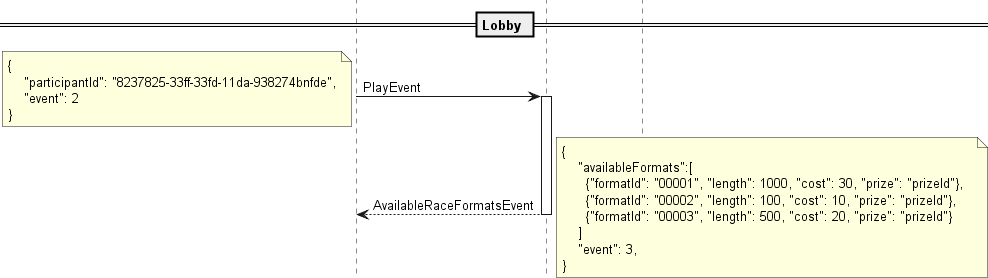
\includegraphics[width=14.5cm]{figure/RacesFormats.png}
            \caption{Diagramma di sequenza per gli eventi GetAvailableRacesEvent e OnAvailableRacesFormatsEvent}
            \label{img:PlayEvent}
        \end{figure}

        \subsubsection{JoinEvent e PlayerJoinedEvent}

        \begin{figure}[!ht]
            \centering
            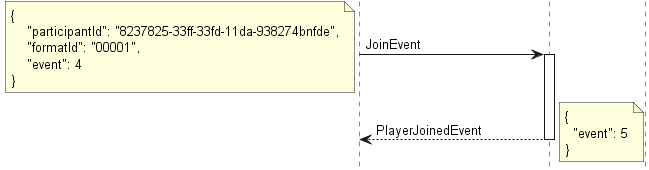
\includegraphics[width=13cm]{figure/JoinEvent.png}
            \caption{Diagramma di sequenza per gli eventi JoinEvent e PlayerJoinedEvent}
        \end{figure}

        \subsubsection{StartingGridEvent e AnotherPlayerJoinedEvent}

        \begin{figure}[!ht]
            \centering
            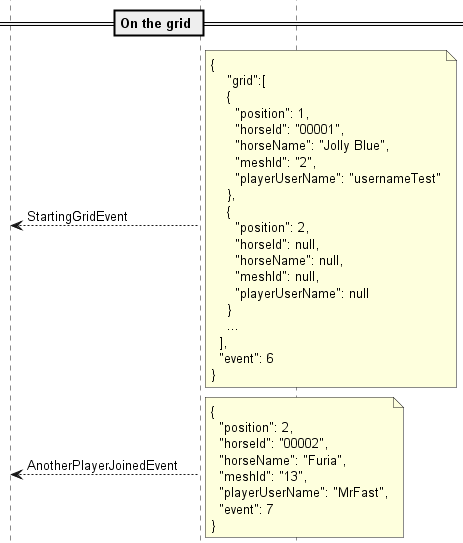
\includegraphics[width=10cm]{figure/StartingGrid.png}
            \caption{Diagramma di sequenza per gli eventi StartingGridEvent e AnotherPlayerJoinedEvent}
        \end{figure}

        \subsubsection{CountdownEvent e RaceEvent}

        \begin{figure}[!ht]
            \centering
            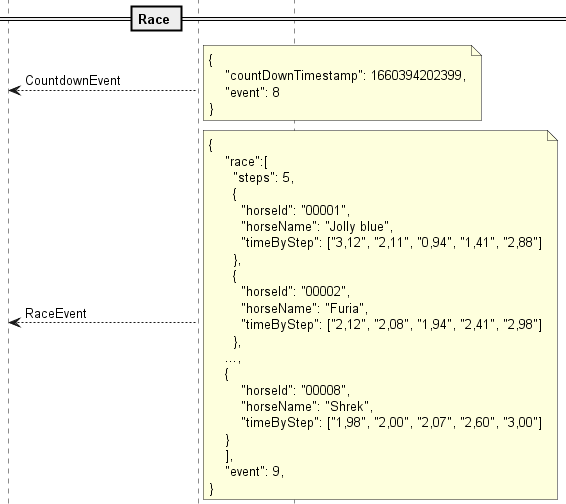
\includegraphics[width=11cm]{figure/CountdownEvent.png}
            \caption{Diagramma di sequenza per gli eventi CountdownEvent e RaceEvent}
        \end{figure}

        \subsubsection{RaceFinishedEvent e Leaderboardevent}

        \begin{figure}[!ht]
            \centering
            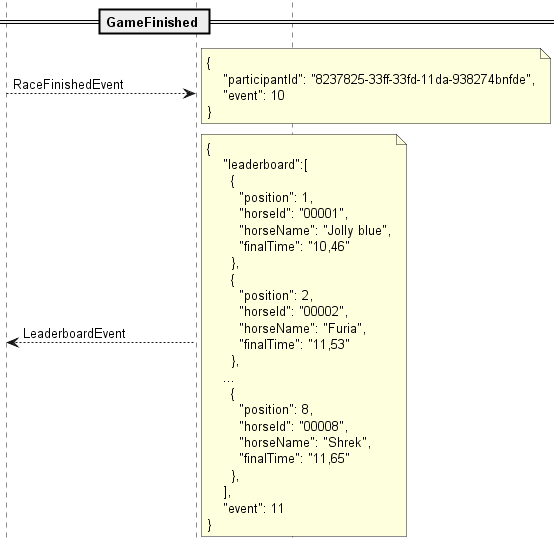
\includegraphics[width=12cm]{figure/RaceFinishedEvent.png}
            \caption{Diagramma di sequenza per gli eventi RaceFinishedEvent e LeaderboardEvent}
        \end{figure}


\section{Scelte di progetto guidate dalla flessibilità}

\section{Programmazione ad Eventi (EDP)}

% Lo metto qui invece che nell'implementazione perché per ora non c'è un'implementazione ma questa cosa è stata comunque nella fase di progettazione

% L'ingegniere prende scelte

% Mettere molti grafici